\chapter{HTSM}

\emph{HTSM (Heuristic Test Strategy Model)} fue creado por James Bach en 1996
para que lo usen los evaluadores profesionales como una colección estructurada
de recordatorios de qué pensar cuando están creando pruebas, divide el
pensamiento de la creación de pruebas en diferentes ejes de análisis, que,
cuando se unen, permiten al evaluador crear una estrategia de prueba
holística\cite{Bach}.

En este capitulo desglosaremos, y describiremos todos sus componentes, de tal
forma que este construya un marco solido para la planificación, y ejecución de
las pruebas de calidad del producto.

\section{Entorno de proyecto}
En esta sección se describirán aquellos factores del contexto que incluyen
recursos necesarios, restricciones, y cualquier otro elemento del proyecto que
debe ser tomado en cuenta para la evaluación.

\subsection{Misión}
La misión del proyecto es:

Evaluar las funcionalidades provistas por \emph{Salesforce} que componen el
modulo de gestión de productos y listas de precios, con el diseño y ejecución de
múltiples técnicas de evaluación, para que de esta manera se pueda garantizar la
calidad del producto para los clientes.

\subsection{Fuentes de Información}
Para evaluar los componentes antes citados, se encontraron las siguientes
fuentes de información respecto al producto:

\begin{description}
\item [Centro de Ayuda] \emph{Salesforce} ofrece un amplio conjunto de
documentación, información general, preguntas frecuentes, y contacto con el
servicio de asistencia técnica desde su sitio de ayuda
(https://help.salesforce.com/).

Estos recursos serán útiles para conocer las reclamaciones de los usuarios, las
características criticas del producto, y las estrategias del fabricante hacia
sus clientes.

\item [Centro de Desarrollo] \emph{Salesforce} también posee un sitio web
específicamente para compartir recursos de desarrollo sobre la plataforma
(https://developer.salesforce.com/).

Este sitio se podrá aprovechar para consultar las referencias a las API del
servicio, conocer acerca de los componentes y como pueden aprovecharse desde la
perspectiva del desarrollador.

\item [Recursos para administradores] Sitio web enfocado a ofrecer experiencias,
vídeos, herramientas, y un sin fin de recursos orientados a usuarios con el rol
de administración de recursos sobre la plataforma
(https://admin.salesforce.com/resources).

\item [Comunidad \emph{Trailblazer}] Sitio web enfocado a conectar a miembros de
la comunidad \emph{Salesforce}, para compartir experiencias, aprender, y proveer
de nuevas ideas sobre la utilización del servicio
(https://success.salesforce.com/).

\end{description}

\subsection{Equipamiento}
En esta sección describiremos la recursos necesarios para la ejecución del
proyecto.

\subsubsection{Software}
\emph{Salesforce} cuenta con múltiples ediciones que comparten una apariencia,
pero varían según la funcionalidad y los precios. Algunos clientes comienzan con
una edición básica y actualizan a una edición más rica en características a
medida que evolucionan los requisitos empresariales.

En el cuadro \ref{ediciones} se describen las ediciones
disponibles\footnote{Información extraída y disponible en:
https://help.salesforce.com/articleView?id=overview\_edition.htm}.

\begin{table}
\centering
\begin{tabular}{|l|p{9.0cm}|}
\hline
\textbf{Edición} & \textbf{Descripción} \\
\hline
\emph{Essentials} & Herramienta para la elaboración de los mapas mentales. \\
\emph{Professional} & Herramienta para la generación de pruebas combinatorias. \\
\emph{Enterprise} & Herramienta para la solicitud de peticiones HTTP para el uso de API.\\
\emph{Unlimited} & Herramienta basada en web que facilita el proceso de gestión de calidad de software. \\
\emph{Developer} & Servicio de almacenamiento y versionado de código fuente y documentación. \\
\hline
\end{tabular}
\caption{Ediciones actualmente disponibles de Sales Cloud.}
\label{ediciones}
\end{table}

Una característica actual de \emph{Salesforce} es que cuenta con dos interfaces
web diferentes, la antigua conocida como: \emph{Salesforce Classic}, y la nueva
incluida desde 2015 denominada: \emph{Salesforce Lightning}; que tiene como
objetivo principal la unificación del \emph{Look and Feel} a través de todo el
servicio sea cual sea el dispositivo que el cliente utilice\cite{McCarthy}.

Se evaluarán las funcionalidades de los módulos sobre el navegador cuya
participación en el mercado es la mayor, en este caso: \emph{Google Chrome}
como puede verse en la figura \ref{software}.

\begin{figure}
\centering
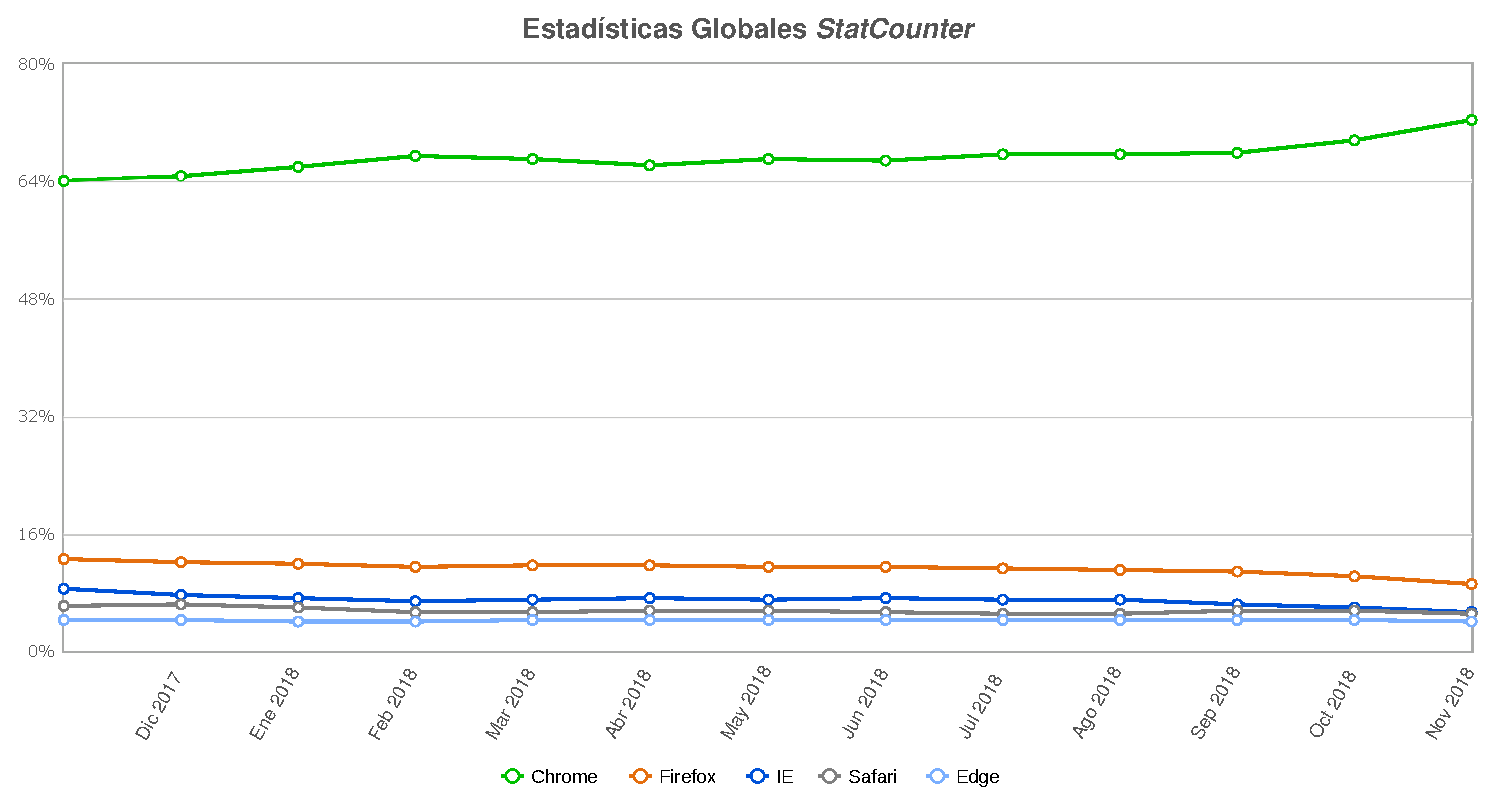
\includegraphics[width=1.0\textwidth]{graphics/compatibilidad.eps}
\caption{Participación de mercado de los navegadores hasta Noviembre del 2018.}
\label{software}
\end{figure}

Adicionalmente se utilizaran algunos navegadores más en pruebas muy focalizadas
de compatibilidad. A partir de la información disponible en la pagina de soporte
provista por el fabricante. Como puede verse en el cuadro
\ref{soporte_navegadores}\footnote{Información extraída y disponible en:
https://help.salesforce.com/articleView?id=getstart\_browsers\_sfx.htm}.

\begin{table}
\centering
\begin{tabular}{|p{4.5cm}|p{1.9cm}|p{1.9cm}|p{1.9cm}|p{1.9cm}|p{1.9cm}|}
\hline
& \textbf{Microsoft Internet Explorer} & \textbf{Microsoft Edge} & \textbf{Google Chrome} & \textbf{Mozilla Firefox} & \textbf{Apple Safari} \\
\hline
Lightning Experience & IE11 (EOL Diciembre 31, 2020) & Ultima versión & Ultima versión & Ultima versión & 11.x+ \\
Lightning Communities & IE11 (EOL Diciembre 31, 2020) & Ultima versión & Ultima versión & Ultima versión & 11.x+ \\
¿Consideraciones especiales de configuración? & No & No & No & No & No \\
Limitaciones conocidas & Sí & Si & No & Si & Si \\
\hline
\end{tabular}
\caption{Lista de Compatibilidad provista por Salesforce.}
\label{soporte_navegadores}
\end{table}

\subsubsection{Herramientas}
En diferentes etapas del proyecto se utilizaran múltiples herramientas que
colaboren con tareas especificas del proceso de evaluación, ellas detalladas en
el cuadro \ref{herramientas}.

\begin{table}
\centering
\begin{tabular}{|l|p{13.5cm}|}
\hline
\textbf{Herramienta} & \textbf{Descripción} \\
\hline
\emph{XMind} & Herramienta para la elaboración de los mapas mentales. \\
\emph{GitHub.com} & Servicio de almacenamiento y versionado de código fuente y documentación. \\
\emph{Testlink} & Herramienta basada en web que facilita el proceso de gestión de calidad de software. \\
\emph{LambdaTest} & Herramienta basada en web para realizar la evaluación de compatibilidad en navegadores. \\
\emph{Pairwise} & Herramienta para la generación de pruebas combinatorias. \\
\emph{Postman} & Herramienta para la solicitud de peticiones HTTP para el uso de API.\\
\hline
\end{tabular}
\caption{Herramientas auxiliares de apoyo para el proyecto.}
\label{herramientas}
\end{table}

\subsection{Cronograma}
Véase el cuadro \ref{cronograma} en la página \pageref{cronograma}.

\begin{sidewaystable}
\centering
\small
\begin{tabular}{|l|l|p{6.5cm}|l|}
\hline
Objetivo General & Objetivos Específicos & Actividades & Resultados \\
\hline
\multirow{15}{4.0cm}{Evaluar el grado de eficacia y eficiencia de los módulos de productos y listas de precios para garantizar la calidad del servicio hacia el cliente.} &
\multirow{3}{4.0cm}{Evaluar las funciones del módulo de gestión de productos para garantizar sus atributos de calidad.} &
Recolectar información, explorar y analizar el módulo de productos. &
\multirow{3}{4.0cm}{Batería de pruebas de evaluación del modulo de productos.} \\
\cline{3-3}
& & Diseñar los tipos de evaluación requeridos para el módulo de productos. & \\
\cline{3-3}
& & Construir la batería de pruebas necesarias para el módulo de productos. & \\
\cline{2-4}
& \multirow{3}{4.0cm}{Evaluar las funciones del módulo de gestión de listas de precios para garantizar sus atributos de calidad.} &
Recolectar información, explorar y analizar el módulo de listas de precios. &
\multirow{3}{4.0cm}{Batería de pruebas de evaluación del modulo de listas de precios.} \\
\cline{3-3}
& & Diseñar los tipos de evaluación requeridos para el módulo de listas de precios. & \\
\cline{3-3}
& & Construir la batería de pruebas necesarias para el módulo de listas de precios. & \\
\cline{2-4}
& \multirow{3}{4.0cm}{Evaluar las características de localización, compatibilidad, y calidad del soporte ofrecido.} &
Explorar, analizar, diseñar y construir una batería de pruebas de localización para los módulos a evaluar. &
\multirow{3}{4.0cm}{Batería de pruebas de localización, compatibilidad, y soportabilidad.} \\
\cline{3-3}
& & Explorar, analizar, diseñar y construir una batería de pruebas de compatibilidad para los módulos a evaluar. & \\
\cline{3-3}
& & Explorar, analizar, diseñar y construir una batería de pruebas de soportabilidad para los módulos a evaluar. & \\
\cline{2-4}
& \multirow{3}{4.0cm}{Evaluar el comportamiento del API disponible del servicio, relativo a productos y listas de precios.} &
Recolectar información, explorar, y analizar las peticiones disponibles en el servicio que comprenden el módulo a evaluar. &
\multirow{3}{4.0cm}{Batería de pruebas automatizadas sobre el API disponible.} \\
\cline{3-3}
& & Diseñar los tipos de evaluación requeridos para el API disponible. & \\
\cline{3-3}
& & Construir y automatizar la batería de pruebas necesarias para la evaluación del API. & \\
\cline{2-4}
& \multirow{3}{4.0cm}{Ejecutar las baterías de pruebas construidas para garantizar la calidad general de los componentes evaluados.} &
Realizar la ejecución de las pruebas manuales. &
\multirow{3}{4.0cm}{Informe de ejecución de pruebas.} \\
\cline{3-3}
& & Realizar la ejecución de las pruebas automatizadas. & \\
\cline{3-3}
& & Analizar y construir estadísticas finales de la evaluación. & \\
\hline
\end{tabular}
\caption{Cronograma de actividades del proyecto.}
\label{cronograma}
\end{sidewaystable}

\subsection{Elementos a evaluar}
Los elementos que se evaluarán los siguientes:

\begin{itemize}
\item Productos.
\item Precios de productos.
\item Listas de precios.
\end{itemize}

La evaluación se realizará a la plataforma, mediante la utilización del navegador
web Google Chrome en su versión 68.0, con excepción de las pruebas automatizadas
que serán ejecutadas mediante scripts de automatización, y las pruebas de
compatibilidad que requerirán muchos navegadores para su evaluación.

\subsection{Documentos entregables}
A continuación se describen los documentos resultantes de la evaluación:

\begin{description}
\item [HTSM] Documento de describe todos los elementos necesarios par la creación
    de pruebas.
\item [Batería de casos de prueba] Conjunto de pruebas a realizar para garantizar
    la calidad del producto.
\item [Batería de reportes de error] Conjunto de reportes de error, generados de
    cualquier problema encontrado en el proceso de ejecución de las pruebas.
\item [Matriz de trazabilidad] Documento que describe la Relación de cobertura
    de las funcionalidades a evaluar con los casos de prueba diseñados.
\item [Scripts de automatización] Código fuente de los programas que se encargan
    de la automatización de las pruebas sobre el API del servicio.
\item [Resultados de ejecución] Informe técnico que condensa los resultados
    finales de la ejecución de las pruebas.
\end{description}

\section{Elementos del producto}
Dentro del alcance de la evaluación se encuentran los componentes de productos
y listas de precios, las funcionalidades que comprenden estos se detallan en
esta sección.

Se considero la interfaz \emph{Lightning Experience}, como único objetivo de la
evaluación. La versión \emph{Lightning Experience} esta disponible para las
siguientes ediciones del producto: \emph{Essentials}, \emph{Group},
\emph{Professional}, \emph{Enterprise}, \emph{Performance}, \emph{Unlimited}, y
\emph{Developer}.

\subsection{Productos}
En la figura \ref{productos} pueden verse las funcionalidades clasificadas desde
la perspectiva de la interfaz de usuario, en ambos componentes se tienen la
parte de los controles de vista de lista similares, por lo que se prefirió
describir esas funciones a una estructura posterior.

\begin{figure}
\centering
\begin{tikzpicture}[
    grow via three points={one child at (0.5,-0.7) and
    two children at (0.5,-0.7) and (0.5,-1.4)},
    edge from parent path={(\tikzparentnode.south) |- (\tikzchildnode.west)}]
    \node {Productos}
        child [missing] {}
        child { node {Filtrar por: Vista de Lista}}
        child { node {Nuevo}}
        child { node {Buscar: Producto}}
        child { node {Controles de Vista de Lista}
            child { node {\ldots}}
        }
        child [missing] {}
        child { node {Mostrar como}}
        child { node {Actualizar}}
        child { node {Modificar Lista}}
        child { node {Lista de Productos}
            child [missing] {}
            child { node {Ver: Producto}
                child [missing] {}
                child { node {Modificar}}
                child { node {Eliminar}}
                child { node {Duplicar}}
                child { node {Relacionado}
                    child [missing] {}
                    child { node {Agregar precio estándar}}
                    child { node {Agregar a lista de precios}}
                    child { node {Ver: Lista de precios}}
                    child { node {Modificar: Lista de precios}}
                    child { node {Eliminar: Lista de precios}}
                    child { node {Ver todos}}
                }
                child [missing] {}
                child [missing] {}
                child [missing] {}
                child [missing] {}
                child [missing] {}
                child [missing] {}
                child [missing] {}
                child { node {Detalles}}
            }
            child [missing] {}
            child [missing] {}
            child [missing] {}
            child [missing] {}
            child [missing] {}
            child [missing] {}
            child [missing] {}
            child [missing] {}
            child [missing] {}
            child [missing] {}
            child [missing] {}
            child [missing] {}
            child [missing] {}
            child [missing] {}
            child { node {Modificar: Producto}}
            child { node {Eliminar: Producto}}
        };
\end{tikzpicture}
\caption{Funciones que componen el módulo de gestión de productos.}
\label{productos}
\end{figure}

Esta clasificación de las funciones se ubican en una vista de interfaz como
puede verse en la figura \ref{productos_web}, vista principal para la gestión
de productos en el servicio.

\begin{figure}
\centering
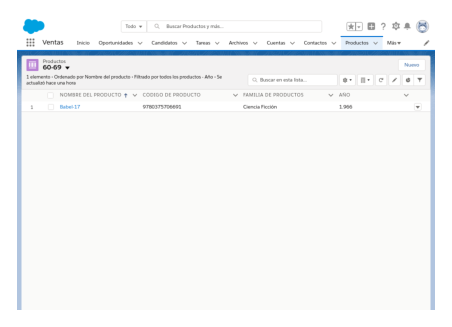
\includegraphics[width=1.0\textwidth]{graphics/productos.eps}
\caption{Interfaz gráfica para el módulo de productos.}
\label{productos_web}
\end{figure}

Para la evaluación de estas funcionalidades se realizarán las siguientes
evaluaciones:

\begin{itemize}
\item \textbf{Pruebas de aceptación}, para las funcionalidades de tipo CRUD en
    el gestor de productos, es decir, creación, visualización, modificación y
    eliminación.
\item \textbf{Pruebas funcionales}, para todos los elementos que están provistos
    por la misma interfaz de usuario.
\item \textbf{Pruebas de dominio}, para los cuatro formularios que maneja el
    gestor de productos, los cuales pueden verse en la figura \ref{productos_formularios}.
\item \textbf{Pruebas negativas}, para la evaluación de los mensajes de
    error provistos por este componente.
\end{itemize}

\begin{figure}
\centering
\begin{tikzpicture}[
    grow via three points={one child at (0.5,-0.7) and
    two children at (0.5,-0.7) and (0.5,-1.4)},
    edge from parent path={(\tikzparentnode.south) |- (\tikzchildnode.west)}]
    \node {Productos}
        child [missing] {}
        child { node {Crear producto}
            child { node {Nombre del producto (*)}}
            child { node {Activo}}
            child { node {Código de producto}}
            child { node {Familia de productos}}
            child { node {Descripción del producto}}
        }
        child [missing] {}
        child [missing] {}
        child [missing] {}
        child [missing] {}
        child [missing] {}
        child [missing] {}
        child { node {Crear entrada del catálogo de precios}
            child { node {Producto (*)}}
            child { node {Activo}}
            child { node {Lista de precios (*)}}
            child { node {Precio de la lista (*)}}
            child { node {Utilizar precio estándar}}
        }
        child [missing] {}
        child [missing] {}
        child [missing] {}
        child [missing] {}
        child [missing] {}
        child [missing] {}
        child { node {Agregar a lista de precios}
            child { node {Lista de precios (*)}}
            child { node {Divisa (*)}}
        }
        child [missing] {}
        child [missing] {}
        child [missing] {}
        child { node {Modificar entrada del catálogo de precios}
            child { node {Activo}}
            child { node {Precio de la lista}}
            child { node {Utilizar precio estándar}}
        };
\end{tikzpicture}
\caption{Formularios que componen el módulo de gestión de productos.}
\label{productos_formularios}
\end{figure}

\subsection{Listas de Precios}
En la figura \ref{listas_de_precios} pueden verse las funcionalidades
clasificadas desde la perspectiva de la interfaz de usuario, también se omitió
la sección de los controles de vista de lista.

\begin{figure}
\centering
\begin{tikzpicture}[
    grow via three points={one child at (0.5,-0.7) and
    two children at (0.5,-0.7) and (0.5,-1.4)},
    edge from parent path={(\tikzparentnode.south) |- (\tikzchildnode.west)}]
    \node {Listas de Precios}
        child [missing] {}
        child { node {Filtrar por: Vista de Lista}}
        child { node {Nuevo}}
        child { node {Buscar: Lista de precios}}
        child { node {Controles de Vista de Lista}
            child { node {\ldots}}
        }
        child [missing] {}
        child { node {Mostrar como}}
        child { node {Actualizar}}
        child { node {Modificar Lista}}
        child { node {Lista de Listas de Precios}
            child [missing] {}
            child { node {Ver: Lista de precios}
                child [missing] {}
                child { node {Modificar}}
                child { node {Eliminar}}
                child { node {Duplicar}}
                child { node {Relacionado}
                    child [missing] {}
                    child { node {Agregar productos}}
                    child { node {Ver: Producto}}
                    child { node {Modificar: Producto}}
                    child { node {Eliminar: Producto}}
                    child { node {Ver todos}}
                    child { node {Historial de lista de precios (Ver todos)}}
                }
                child [missing] {}
                child [missing] {}
                child [missing] {}
                child [missing] {}
                child [missing] {}
                child [missing] {}
                child [missing] {}
                child { node {Detalles}}
            }
            child [missing] {}
            child [missing] {}
            child [missing] {}
            child [missing] {}
            child [missing] {}
            child [missing] {}
            child [missing] {}
            child [missing] {}
            child [missing] {}
            child [missing] {}
            child [missing] {}
            child [missing] {}
            child [missing] {}
            child [missing] {}
            child { node {Modificar: Lista de Precios}}
            child { node {Eliminar: Lista de Precios}}
        };
\end{tikzpicture}
\caption{Funciones que componen el módulo de gestión de listas de precios.}
\label{listas_de_precios}
\end{figure}

Esta clasificación de las funciones se ubican en una vista de interfaz como
puede verse en la figura \ref{listas_de_precios_web}, vista principal para la
gestión de listas de precios en el servicio.

\begin{figure}
\centering
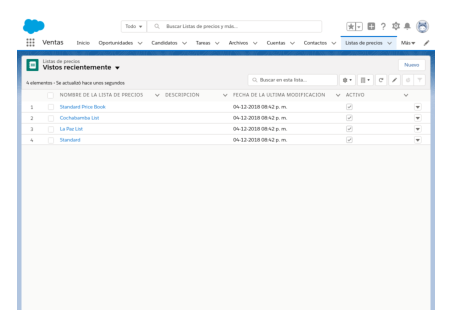
\includegraphics[width=1.0\textwidth]{graphics/listas_de_precios.eps}
\caption{Interfaz gráfica para el módulo de listas de precios.}
\label{listas_de_precios_web}
\end{figure}

Para la evaluación de estas funcionalidades se realizarán las siguientes
evaluaciones:

\begin{itemize}
\item \textbf{Pruebas de aceptación}, para las funcionalidades de tipo CRUD en
    el gestor de listas de precios, es decir, creación, visualización,
    modificación y eliminación.
\item \textbf{Pruebas funcionales}, para todos los elementos que están provistos
    por la misma interfaz de usuario.
\item \textbf{Pruebas de dominio}, para los dos formularios que maneja el
    gestor de productos, los cuales pueden verse en la figura \ref{listas_de_precios_formularios}.
\item \textbf{Pruebas negativas}, para la evaluación de los mensajes de error
    provistos por este componente.
\end{itemize}

\begin{figure}
\centering
\begin{tikzpicture}[
    grow via three points={one child at (0.5,-0.7) and
    two children at (0.5,-0.7) and (0.5,-1.4)},
    edge from parent path={(\tikzparentnode.south) |- (\tikzchildnode.west)}]
    \node {Listas de precios}
        child [missing] {}
        child { node {Crear lista de precios}
            child { node {Nombre de la lista de precios}}
            child { node {Activo}}
            child { node {Descripción}}
            child { node {Es lista de precios estándar}}
        }
        child [missing] {}
        child [missing] {}
        child [missing] {}
        child [missing] {}
        child [missing] {}
        child { node {Agregar productos}
            child { node {Buscar entrada de catálogos de precios}}
        };
\end{tikzpicture}
\caption{Formularios que componen el módulo de gestión de listas de precios.}
\label{listas_de_precios_formularios}
\end{figure}

\subsection{Controles de Vista de Lista}
En la figura \ref{vista_de_lista} pueden verse las funciones omitidas en los
diagramas anteriores relativas a los controles de vista, ambas equivalentes
entre si.

\begin{figure}
\centering
\begin{tikzpicture}[
    grow via three points={one child at (0.5,-0.7) and
    two children at (0.5,-0.7) and (0.5,-1.4)},
    edge from parent path={(\tikzparentnode.south) |- (\tikzchildnode.west)}]
    \node {Controles de Vista de Lista}
        child [missing] {}
        child { node {Duplicar}}
        child { node {Cambiar nombre}}
        child { node {Configuración de colaboración}}
        child { node {Modificar filtros de lista}
            child [missing] {}
            child { node {Ver/Modificar: Filtro}}
            child { node {Eliminar: Filtro}}
            child { node {Agregar Filtro}}
            child { node {Eliminar todos}}
            child { node {Agregar lógica de filtro}}
        }
        child [missing] {}
        child [missing] {}
        child [missing] {}
        child [missing] {}
        child [missing] {}
        child [missing] {}
        child [missing] {}
        child { node {Seleccionar los campos que se visualizaran}}
        child { node {Eliminar}}
        child { node {Restablecer anchuras de columna}};
\end{tikzpicture}
\caption{Funciones que componen el módulo de gestión de vistas de lista.}
\label{vista_de_lista}
\end{figure}

Para la evaluación de estas funcionalidades se realizarán las siguientes
evaluaciones:

\begin{itemize}
\item \textbf{Pruebas de aceptación}, para las funcionalidades de tipo CRUD en
    el gestor de vistas de lista, es decir, creación, visualización,
    modificación y eliminación.
\item \textbf{Pruebas funcionales}, para todos los elementos que están provistos
    por la misma interfaz de usuario.
\item \textbf{Pruebas de dominio}, para los seis formularios que maneja el
    gestor de vistas de lista, los cuales pueden verse en la figura
    \ref{vista_de_lista_formularios}.
\item \textbf{Pruebas negativas}, para la evaluación de los mensajes de
    error provistos por este componente.
\end{itemize}

\begin{figure}
\centering
\begin{tikzpicture}[
    grow via three points={one child at (0.5,-0.7) and
    two children at (0.5,-0.7) and (0.5,-1.4)},
    edge from parent path={(\tikzparentnode.south) |- (\tikzchildnode.west)}]
    \node {Vista de lista}
        child [missing] {}
        child { node {Nueva vista de lista}
            child { node {Nombre de la lista}}
            child { node {List API Name}}
            child { node {¿Quien ve esta vista de lista?}
                child { node {Solo yo puedo ver esta vista de lista}}
                child { node {Todos los usuarios pueden ver esta vista de lista}}
                child { node {Compartir vista de lista con grupos de usuarios}}
            }
        }
        child [missing] {}
        child [missing] {}
        child [missing] {}
        child [missing] {}
        child [missing] {}
        child [missing] {}
        child [missing] {}
        child { node {Cambiar nombre}
            child { node {Nombre de lista}}
            child { node {List API Name}}
        }
        child [missing] {}
        child [missing] {}
        child [missing] {}
        child { node {Configuración de colaboración}
            child { node {¿Quien ve esta vista de lista?}
                child { node {Solo yo puedo ver esta vista de lista}}
                child { node {Todos los usuarios pueden ver esta vista de lista}}
                child { node {Compartir vista de lista con grupos de usuarios}}
            }
        }
        child [missing] {}
        child [missing] {}
        child { node {Agregar filtro}
            child { node {Campo}}
            child { node {Operador}}
            child { node {Valor}}
        }
        child [missing] {}
        child [missing] {}
        child [missing] {}
        child [missing] {}
        child { node {Agregar lógica de filtro}
            child { node {Lógica de filtro}}
        }
        child [missing] {}
        child [missing] {}
        child { node {Seleccionar los campos que se visualizaran}
            child { node {Campos disponibles}}
            child { node {Campos visibles}}
        };
\end{tikzpicture}
\caption{Formularios que componen el módulo de gestión de vistas de listas.}
\label{vista_de_lista_formularios}
\end{figure}

\section{Técnicas de prueba}
Habiéndose definido los elementos del sistema, y los criterios bajo los que
estos deben ser evaluados. Ahora se pasará a describir las técnicas de prueba
que se utilizarán para cada elemento y criterio de calidad.

\subsection{Pruebas de aceptación}
La prueba de aceptación es una prueba formal que se realiza para determinar si
un sistema satisface sus criterios de aceptación: los criterios que debe cumplir
el sistema para que el cliente los acepte. Ayuda al cliente a determinar si
acepta o no el sistema\cite{Naik}.

Las pruebas de aceptación se realizaron para los tres componentes que comprenden
el alcance del proyecto, como el mínimo de las funcionalidades que se consideran
criticas, en este caso, las operaciones de creación, visualización, modificación
y eliminación de los elementos de cada componente.

Se crearon 55 casos de prueba, que pueden consultarse en los anexos de este
documento, siendo cada caso de prueba como el que se muestra en la figura
\ref{tc_acceptance}.

\begin{figure}
\centering
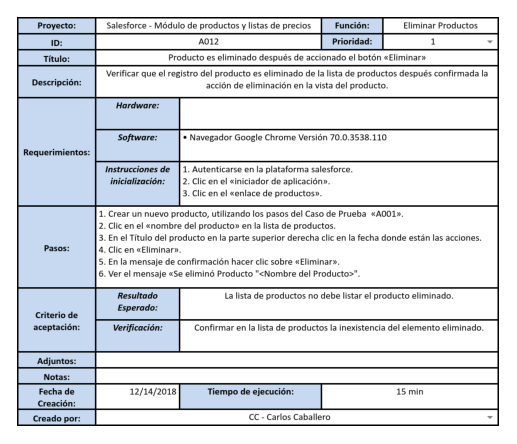
\includegraphics[width=1.0\textwidth]{graphics/tc1-acceptance.eps}
\caption{Caso de Prueba de Aceptación.}
\label{tc_acceptance}
\end{figure}

\subsection{Pruebas funcionales}
El software o sistema bajo prueba se ve como una «caja negra». La selección de
casos de prueba para pruebas funcionales se basa en el requisito o
especificación de diseño de la entidad de software bajo prueba. Ejemplos de
resultados esperados, algunas veces se llaman oráculos de prueba, incluyen
requisitos/especificaciones de diseño, valores calculados a mano y resultados
simulados. Las pruebas funcionales hacen hincapié en el comportamiento externo
de la entidad de software\cite{Luo}.

Las pruebas funcionales se realizaron para cada acción encontrada en la interfaz
de usuario, siendo barrido completamente cualquier operación disponible en los
componentes a evaluar.

Se crearon 144 casos de prueba, que pueden consultarse en los anexos de este
documento, siendo cada caso de prueba como el que se muestra en la figura
\ref{tc_functional}.

\begin{figure}
\centering
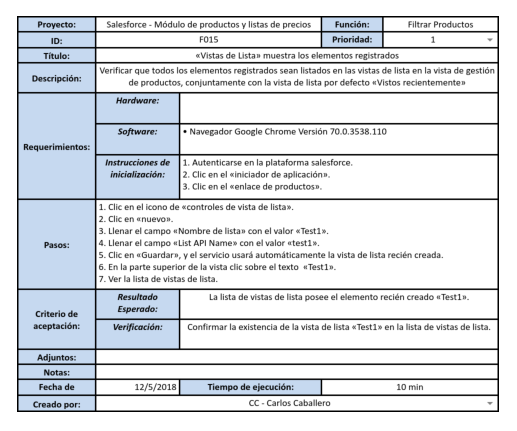
\includegraphics[width=1.0\textwidth]{graphics/tc2-functional.eps}
\caption{Caso de Prueba Funcional.}
\label{tc_functional}
\end{figure}

\subsection{Pruebas de dominio}
La prueba de dominio es una estrategia de muestreo estratificada para elegir
algunos casos de prueba de la infinidad de casos de prueba candidatos. La
estrategia tiene varios nombres, como la partición de equivalencia, el análisis
de límites y la partición de categorías.

La prueba de dominio es probablemente la más ampliamente descrita y una de las
técnicas de prueba de software más ampliamente practicadas. Algunos autores
restringen su consideración del alcance de esta técnica a variables de entrada
linealizables a funciones matemáticas. Una variable linealizable es aquella
cuyos valores se pueden asignar a una recta numérica. El análisis es más
sencillo y más obvio en estos casos\cite{Kaner}.

\subsection{Pruebas negativas}
La prueba negativa, comúnmente conocida como \emph{prueba de ruta de error} o
\emph{prueba de falla}, generalmente se realiza para garantizar la estabilidad
de la aplicación.

La prueba negativa es el proceso de aplicar tanta creatividad como sea posible y
validar la aplicación contra datos no válidos. Esto significa que su propósito
es verificar si los errores se muestran al usuario donde se supone que debe
hacerlo o si se está manejando un valor incorrecto con mayor gracia.

La fiabilidad funcional de la aplicación o el software solo se puede cuantificar
con escenarios negativos diseñados de manera efectiva. Las pruebas negativas no
solo apuntan a detectar fallas potenciales que podrían causar un impacto grave
en el consumo del servicio, sino que también pueden ser fundamentales para
determinar las condiciones bajo las cuales la aplicación puede fallar.
Finalmente, garantiza que haya suficiente validación de errores presente en el
software\cite{Nadig}.

Las pruebas negativas se centraron en los mensajes de errores que el sistema
envía y debe enviar según los mismos criterios del producto.

Se crearon 25 casos de prueba, que pueden consultarse en los anexos de este
documento, siendo cada caso de prueba como el que se muestra en la figura
\ref{tc_negative}.

\begin{figure}
\centering
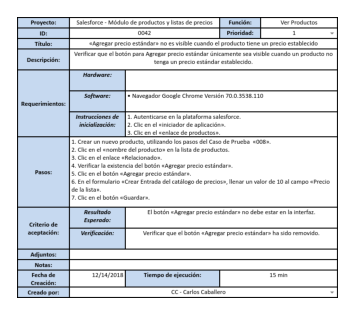
\includegraphics[width=1.0\textwidth]{graphics/tc3-negative.eps}
\caption{Caso de Prueba Negativa.}
\label{tc_negative}
\end{figure}

\subsection{Pruebas de compatibilidad}
La prueba de compatibilidad es una prueba no funcional realizada en la
aplicación para evaluar la compatibilidad de la aplicación en diferentes
entornos. En este caso sobre diferentes navegadores.

\subsection{Pruebas de localización}
El propósito de las pruebas de localización es asegurar que los errores no se
hayan introducido durante el proceso de traducción, que el contenido traducido
se muestre correctamente y que el producto localizado funcione como se espera
para el mercado objetivo. Probar sitios web para garantizar la adaptabilidad a
un lugar y una cultura en particular también es crucial para sugerir su
superioridad en el mercado objetivo\cite{Sampair}.

Aquí hay algunas áreas que examinamos durante esta prueba:

\begin{itemize}
\item Todos los recursos de localización están traducidos correctamente.
\item La compilación generada incluye todos los archivos necesarios.
\item La funcionalidad en la versión localizada es consistente con el producto de origen.
\item La pantalla localizada tiene el mismo número y tipo de elementos que el del producto de origen.
\item Todos los caracteres específicos del entorno local aparecen correctamente.
\item No hay palabras que pasen sobre los botones o se corten en la página.
\end{itemize}

\section{Criterios de calidad}
Se denomina criterio de calidad a cualquier requerimiento que define lo que el
producto debe ser.

Por lo general, los criterios de calidad parten de la combinación de las
necesidades reales y de las demandas de los clientes, con el conocimiento de las
ofertas y productos de organizaciones de la competencia y las posibilidades que
el fabricante posee para satisfacer esas necesidades y expectativas o para
procurar en la medida de lo posible y/o aconsejable\cite{Haaz}.

Se definieron los siguientes como criterios de calidad fundamentales para el
éxito del producto\cite{Fillottrani}.

\begin{description}
\item [Usabilidad] La usabilidad se refiere a la facilidad de operación del
    producto por parte de los usuarios, y se relaciona con el esfuerzo
    necesario para ser utilizado, y en la evaluación individual de tal uso, por
    parte de un conjunto especificado o implícito de usuarios.

    Entre algunos de los criterios que determinan este factor, están:

    \begin{itemize}
    \item \textbf{Entendimiento} que mide el esfuerzo del usuario en reconocer el
        concepto lógico del software y su aplicabilidad.
    \item \textbf{Aprendizaje} que mide el esfuerzo del usuario en aprender
        acerca del producto.
    \item \textbf{Operabilidad} que mide el esfuerzo del usuario en operar y
        controlar el sistema.
    \end{itemize}

\item [Compatibilidad] La compatibilidad del navegador determina el
    comportamiento del servicio en diferentes plataformas de navegación.

    Dado que cada navegador tiene su propia manera de mostrar y gestionar los
    contenidos de una página web. Por lo tanto, las páginas web deben diseñarse
    de tal manera que puedan ser compatibles con cada uno de los navegadores de
    uso común. Actualmente hay casi cien tipos diferentes de navegadores
    disponibles, lo que dificulta que los diseñadores / webmasters desarrollen
    sitios web con un comportamiento similar en múltiples plataformas. El
    estricto cumplimiento de las pautas de diseño puede cumplir con estos
    criterios hasta cierto nivel.

\item [Soportabilidad] La soportabilidad es la capacidad del sistema para
    proporcionar información útil para identificar y resolver problemas.

    El costo de mantener el atributo de compatibilidad es alto y el resultado
    solo es visible a gran escala. Sin embargo, con el crecimiento del equipo y
    el producto, este atributo se convierte en una de las claves\cite{Ashanin}.

\item [Localizabilidad] La localizabilidad es un proceso intermedio para
    verificar que una aplicación globalizada está lista para la localización.
    En una situación ideal, esta es solo una fase de garantía de calidad. Si se
    diseñó y desarrolló una aplicación con miras a la localización, esta fase
    consistirá principalmente en pruebas de localizabilidad. De lo contrario, es
    durante esta fase que se descubrirán y corregirán los errores en el código
    fuente que impiden la localización.

    La localizabilidad ayuda a garantizar que la localización no introduzca
    ningún defecto funcional en la aplicación\cite{Moura}.
\end{description}

